\documentclass{article}%
\usepackage[T1]{fontenc}%
\usepackage[utf8]{inputenc}%
\usepackage{lmodern}%
\usepackage{textcomp}%
\usepackage{lastpage}%
\usepackage[head=40pt,margin=0.5in,bottom=0.6in]{geometry}%
\usepackage{graphicx}%
%
\title{\textbf{En Anzoátegui piden al fiscal general resolver caso de familiares desaparecidos}}%
\author{MIRIAM RIVERO}%
\date{28/11/2018}%
%
\begin{document}%
\normalsize%
\maketitle%
\textbf{URL: }%
http://www.eluniversal.com/venezuela/26958/en{-}anzoategui{-}piden{-}al{-}fiscal{-}general{-}resolver{-}caso{-}de{-}familiares{-}desaparecidos\newline%
%
\textbf{Periodico: }%
EU, %
ID: %
26958, %
Seccion: %
venezuela\newline%
%
\textbf{Palabras Claves: }%
NO\_TIENE\newline%
%
\textbf{Derecho: }%
1.2, %
Otros Derechos: %
1.10, %
Sub Derechos: %
1.2.5, 1.10.2\newline%
%
\textbf{EP: }%
NO\newline%
\newline%
%
\textbf{\textit{El caso está relacionado con la desaparición física de Marbella Rodríguez Quinan, su hija Yoselín Laya Rodríguez y Oswaldo Vásquez}}%
\newline%
\newline%
%
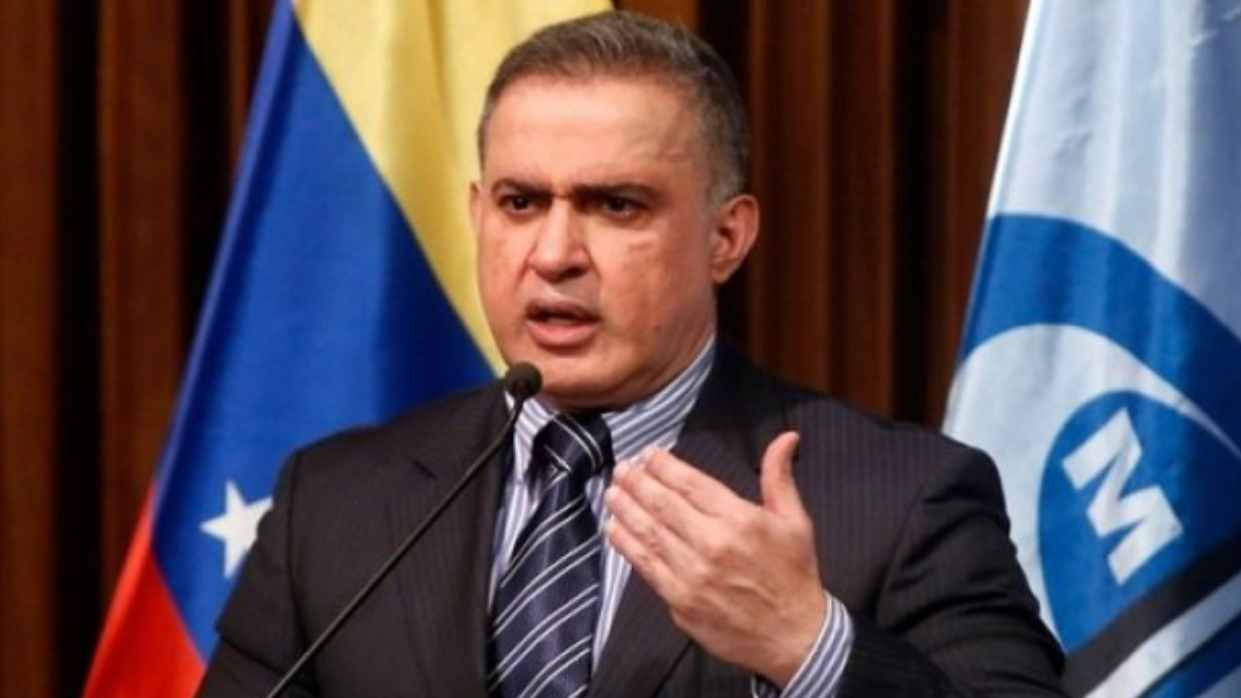
\includegraphics[width=300px]{234.jpg}%
\newline%
%
Puerto La Cruz.{-} Los familiares de tres personas que desaparecieron en noviembre del año 2010 están solicitando al fiscal general de la República, Tarek William Saab, que el despacho que dirige resuelva este caso que mantiene "en zozobra y en incertidumbre" al grupo de sus allegados, que esperan por una respuesta de este ente nacional.%
\newline%
%
El caso está relacionado con la desaparición física de Marbella Rodríguez Quinan, su hija Yoselín Laya Rodríguez y Oswaldo Vásquez, quienes viajaron a Caracas desde Puerto La Cruz el 30 de noviembre y desde ese día no se comunicaron más con sus allegados, según el testimonio de los familiares.%
\newline%
%
Paula Quinan de Rodríguez,  madre de Marbella Rodríguez y abuela de Yoselín Laya, dijo que está desconsolada desde que ocurrió el suceso, "por eso pido de corazón al fiscal general, Tarek William Saab, así como ha resuelto tantos casos de diferentes delitos, desenrede este cangrejo policial, porque se presumen que los tres fueron asesinados, estrangulados y sus cadáveres quemados, por la forma en que aparecieron las osamentas, juntas pero incompletas".%
\newline%
%
Señaló que al cumplirse 8 años del hecho aún no se sabe nada, aun cuando los cuerpos policiales y el Instituto Venezolano de Investigaciones Científicas (IVIC) hicieron pruebas a tres cadáveres que aparecieron debajo del puente de Kempis, estado Miranda, y cuyas características coincidían con las de los desaparecidos.%
\newline%
%
Relató que el día del desafortunado viaje se registró una fuerte precipitación en ese lado de la Troncal 9, que une a Puerto La Cruz con Caracas, y hubo grandes inundaciones que afectaron viviendas y personas y se manejó  inicialmente la tesis de que fueron arrastrados por las aguas. Sin embargo, al aparecer las osamentas de los tres cadáveres, hace tres años, pudo haber cambiado esta versión.%
\newline%
%
La septuagenaria dama, quien reside en el barrio Tierra Adentro de Puerto La Cruz, narró que se enteró por un diario nacional del hallazgo de las osamentas y que en el IVIC  les aplicaron las pruebas de ADN, pero "este organismo aduce que entregó los resultados al Ministerio Público, pero el fiscal del caso dice que faltan otras pruebas, pero no hay  falta el reactivo para hacerlas". El expediente es el número 31542010 y está en la Fiscalía Tercera.%
\newline%
%
La señora Rodríguez Quinan se ha reunido con varios fiscales superiores de Anzoátegui y todos han prometido aclarar este hecho, pero después de diez años nada ha sucedido.%
\newline%
%
"Quiero una respuesta aunque sea la más dura, quiero saber qué paso con mis muchachas", refirió, recodando que Marbella era enfermera profesional y laboraba en el hospital de Guaraguao del IVSS; César Rodríguez y su nieta Yoselín era estudiante de Ingeniería en la UDO Anzoátegui.%
\newline%
%
Mencionó asimismo que el lamentable accidente sucedió cuando el ahora fiscal general era gobernador del estado oriental, por eso pide su apoyo para que se esclarezca el caso.%
\newline%
%
\end{document}